\documentclass[12pt]{article}
\newcommand\tab[1][1cm]{\hspace{#1}}
\usepackage[utf8]{inputenc}
\usepackage{listings}
\usepackage{color}
\usepackage{textcomp}
\usepackage{sectsty}
\usepackage{graphicx}
\pagenumbering{gobble}

\definecolor{codegreen}{rgb}{0,0.6,0}
\definecolor{codegray}{rgb}{0.5,0.5,0.5}
\definecolor{codepurple}{rgb}{0.58,0,0.82}
\definecolor{backcolour}{rgb}{0.95,0.95,0.92}
\sectionfont{\fontsize{12}{15}\selectfont}
\lstdefinestyle{mystyle}{
	backgroundcolor=\color{backcolour},   
	commentstyle=\color{codegreen},
	keywordstyle=\color{magenta},
	numberstyle=\tiny\color{codegray},
	stringstyle=\color{codepurple},
	basicstyle=\footnotesize,
	breakatwhitespace=false,         
	breaklines=true,                 
	captionpos=b,                    
	keepspaces=true,                 
	numbers=left,                    
	numbersep=5pt,                  
	showspaces=false,                
	showstringspaces=false,
	showtabs=false,                  
	tabsize=2
}

\lstset{style=mystyle}


\begin{document}
\author{Eric Pereira\\
	CSE4020: Section 01}
\date{September 13\textsuperscript{th}, 2018}
\title{Assignment 1}
\maketitle


\section{Explain the distinctions among the terms primary key, candidate key, and superkey. Give one example (not presented in class) that includes the three types}
\tab A primary key is one, or a set of attributes, that can uniquely define each entity in a set of entities. A candidate key is one, or a set of attributes that can qualify as a unique minimal key in the database. A primary key can be a candidate key. A superkey is any set of attributes that can uniquely identify a set of entities. a candidate key is a subset of a candidate key, and a superkey can technically be a primary key, although it is more ideal to make the primary key the same as the candidate key. This is, of course, up to the discretion of the designer. 
\section{Explain the difference between a weak and a strong entity set. We can convert any weak entity set to a strong entity set by simply adding appropriate attributes. Why, then, do we have weak entity sets?}
\tab A weak entity set is a is an entity set that that does not have sufficient attributes to form a primary key. A Strong entity key is an entity set that does have sufficient attributes to form a primary key. The reason why we use weak entity sets is useful because it is essentially an extension of a strong entity set, especially for data that is "optional" (similar to the car insurance example in class, where not every car gets into an accident)

\section{Construct an E-R diagram for a hospital with a set of patients and a set of medical doctors. Associate with each patient a log of the various tests and examinations conducted.}
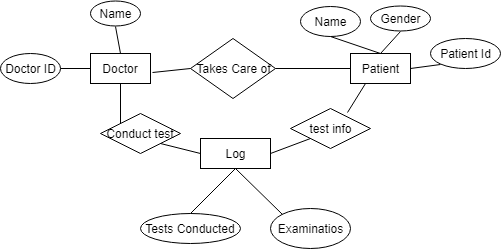
\includegraphics[scale=0.75]{Homeworksss.png}
\section{Give a meaningful example of the need for role indicators in ER diagrams. (Don't give a diagram, just an example in words. Also, don't use the example presented in class)}
\tab Role indicators are used to help describe a relationship that may be between multiple entities in the same entity set. A good example of this is with employees. A company will have managers and workers. A worker needs to report to a manger, who is also an employee, and thus role indicator's can express this more easily. 
\section{Construct an ER diagram for a car insurance company whose customers own one or more cars each. Each car has associated with it zero to any number of recorded accidents. Then, convert the E-R diagram into a set of relational schemas.}
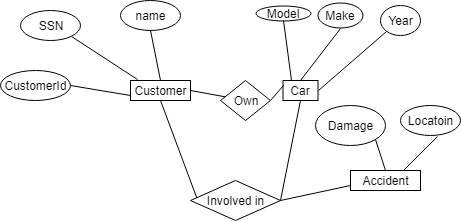
\includegraphics[scale=0.75]{Homeworksssss.png}\\
Schemas: \\
\textit{Customers(CustomerId, SSN, name)} \\
\textit{Vehicle(Make, Model, Year)} \\
\textit{Accident(Damage, Location)}
\section{Construct appropriate E-R diagrams for the following relation schemas. }
\textit{student (ID, name, dept-name, tot-cred)} \\
\tab \textit{course (course-id, title, credits)} \\
\tab \textit{section(course-id, section id, semester, year)} \\
\tab \textit{exam\_marks (student-id, course-id, sec-id, semester, year, exam-id, mark)}
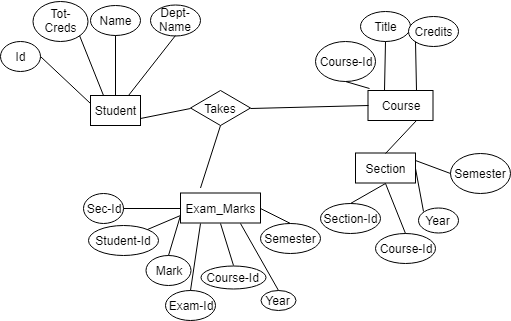
\includegraphics[scale=0.75]{Homeworkssssss.png}
\section{Construct appropriate relation schemas for the following E-R diagrams.}
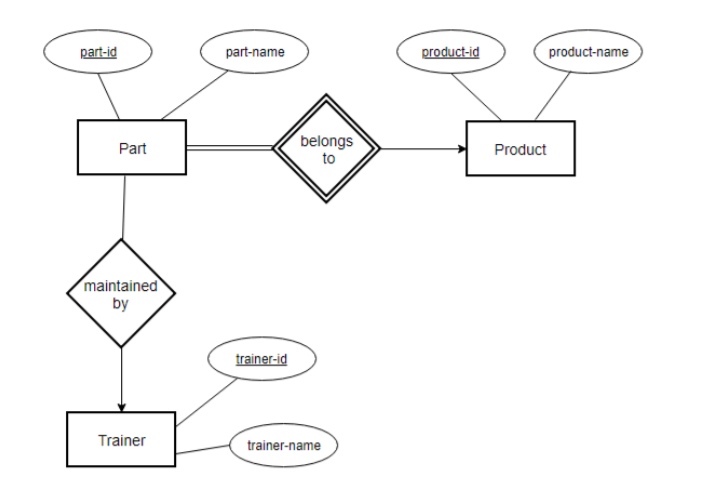
\includegraphics{RelationSchemaPhoto.png}\\
Schemas: \\
\textit{Part(part-id, part-name)}\\
\textit{Trainer(trainer-id, trainer-name)} \\
\textit{Product(product-id, product-name)}
\end{document}